\documentclass[12pt]{exam}

\usepackage[utf8]{inputenc}  % For UTF8 source encoding.
\usepackage{amsmath}  % For displaying math equations.
\usepackage{amsfonts} % For mathematical fonts (like \mathbb{E}!).
\usepackage{upgreek}  % For upright Greek letters, such as \upvarphi.
\usepackage{wasysym}  % For additional glyphs (like \smiley!).
\usepackage{mathrsfs} % For script text (hash families and universes).
\usepackage{enumitem}
\usepackage{graphicx}
% For document margins.
\usepackage[left=.8in, right=.8in, top=1in, bottom=1in]{geometry}
\usepackage{lastpage} % For a reference to the number of pages.
\usepackage[table,xcdraw]{xcolor}
\usepackage{pdfpages}
\usepackage{verbatim}
\usepackage{afterpage}

% TODO: Enter your name here :)
\newcommand*{\authorname}{Luis A. Perez}

\newcommand*{\duedate}{Wednesday, July 17th}
\newcommand*{\duetime}{11:59 pm}

% Fancy headers and footers
\headrule
\firstpageheader{EE 263\\Summer 2019}{Homework 3 \\ }{Due: \duedate\\at \duetime}
\runningheader{EE 263}{Homework 3}{\authorname}
\footer{}{\footnotesize{Page \thepage\ of \pageref{LastPage}}}{}

% Exam questions.
\newcommand{\Q}[1]{\question{\large{\textbf{#1}}}}
\qformat{}  % Remove formatting from exam questions.

% Useful macro commands.
\newcommand*{\bigtheta}[1]{\Theta\left( #1 \right)}
\newcommand*{\bigo}[1]{O \left( #1 \right)}
\newcommand*{\bigomega}[1]{\Omega \left( #1 \right)}
\newcommand*{\prob}[1]{\text{Pr} \left[ #1 \right]}
\newcommand*{\ex}[1]{\text{E} \left[ #1 \right]}
\newcommand*{\var}[1]{\text{Var} \left[ #1 \right]}

\newcommand*{\norm}[1]{\left\lVert #1 \right\rVert}
\newcommand*{\HH}{\mathscr{H}}   % Family of hash functions.
\newcommand*{\UU}{\mathscr{U}}   % Universe.
\newcommand*{\eps}{\varepsilon}  % Epsilon.


% Custom formatting for problem parts.
\renewcommand{\thepartno}{\roman{partno}}
\renewcommand{\partlabel}{\thepartno.}

% Framed answers.
\newcommand{\answerbox}[1]{
\begin{framed}
\hspace{\fill}
\vspace{#1}
\end{framed}}

\printanswers

\setlength\answerlinelength{2in} \setlength\answerskip{0.3in}

\begin{document}
\title{EE 263 Homework 3}
\author{\authorname}
\date{}
\maketitle
\thispagestyle{headandfoot}
\setcounter{MaxMatrixCols}{15}

\begin{questions}
%%%%%%%%%%%%%%%%%%%%%%%%%%%%%%%%%%%
\Q{The smoothest input that takes the state to zero}

  \begin{solution}
    \begin{enumerate}[label=(\alph*)]
      \item We beging by trying to express the problem in a way that's more susceptible to the techniques that we're learned in the course. Firstly, let us simply expand $x(20)$. We have:
      \begin{align*}
        x(20) &= Ax(19) + Bu(19) \tag{Using our recurrence}\\
        &= A(Ax(18) + Bu(18)) + Bu(19) \tag{Re-use reccurence} \\
        &= A^2x(18) + ABu(18) + Bu(19) \tag{Simplify} \\
        &= A^2(Ax(17) + Bu(17)) + ABu(18) + Bu(19) \tag{Apply reccurrences again} \\
        &= A^3x(17) + A^2Bu(17) + ABu(18) + Bu(19) \\
        \vdots \\
        &= A^{20}x(0) + \sum_{i=0}^{19} A^iBu(19 - i) 
      \end{align*}
      We know that $x(20) = 0$, we re-arranginh the above, we have:
      \begin{align*}
        \sum_{i=0}^{19} A^iBu(19-i) &= -A^{20}x(0) \\
        \begin{bmatrix}
          B & AB & A^2B & A^3B & \cdots & A^{19}B
        \end{bmatrix}
        \begin{bmatrix}
          u(19) \\
          u(18) \\
          u(17) \\
          u(16) \\
          \vdots \\
          u(0)
        \end{bmatrix} &= -A^{20}x(0) \\
        Cu &= y
      \end{align*}
      where we have
      \begin{align*}
        C &=
          \begin{bmatrix}
            B & AB & A^2B & \cdots & A^{19}B
          \end{bmatrix} \in \mathbb{R}^{3 \times 20} \\
        u &= 
          \begin{bmatrix}
            u(19) \\
            u(18) \\
            u(17) \\
            \vdots \\
            u(0)
          \end{bmatrix} \in \mathbb{R}^{20}\\
        y &= -A^{20}x(0) \in \mathbb{R}^{3}
      \end{align*}
      with $C$ and $y$ known, and $u$ as the parameters we're trying to find. Note that the above is an underdetermined system of linear equations with 3 equations and 20 variables.

      The problem above would be straight-forward to solve if what our objective did was minimize the norm of $u$. However, we're actually tryining to minize the the smoothesness. So we'll need to do a change of variables. In fact, we propose defining our variables as:
      \begin{align*}
        \begin{bmatrix}
            u(19) \\
            u(18) \\
            u(17) \\
            \vdots \\
            u(1)\\
            u(0)
          \end{bmatrix} &= 
          \begin{bmatrix}
            1 & 1 & 1 & \cdots & 1 & 1 \\
            0 & 1 & 1 & \cdots & 1 & 1 \\
            0 & 0 & 1 & \cdots & 1 & 1 \\
            \vdots & \vdots & \vdots & \vdots & \vdots & \vdots \\
            0 & 0 & 0 & \cdots & 1 & 1 \\
            0 & 0 & 0 & \cdots & 0 & 1
          \end{bmatrix}
          \begin{bmatrix}
            u(19) - u(18) \\
            u(18) - u(17) \\
            u(17) - u(16) \\
            \vdots \\
            u(1) - u(0) \\
            u(0) - u(-1)
          \end{bmatrix} \\
          &= 
          \begin{bmatrix}
            1 & 1 & 1 & \cdots & 1 & 1 \\
            0 & 1 & 1 & \cdots & 1 & 1 \\
            0 & 0 & 1 & \cdots & 1 & 1 \\
            \vdots & \vdots & \vdots & \vdots & \vdots & \vdots \\
            0 & 0 & 0 & \cdots & 1 & 1 \\
            0 & 0 & 0 & \cdots & 0 & 1
          \end{bmatrix}
          \begin{bmatrix}
            \delta(19) \\
            \delta(18) \\
            \delta(17) \\
            \vdots \\
            \delta(1)\\
            \delta(0)
          \end{bmatrix} \\
          &= T\delta
      \end{align*}
      where $T \in \mathbb{R}^{20 \times 20}$ is an upper triangular matrix of $1$s and $\delta \in \mathbb{R}^{20}$ is the differences between each subsequent value. Using these, we can write our problem as:
      \[ 
        (CT)\delta = y
      \]
      And looking at our objective, we have:
      \begin{align*}
        J_{\text{smooth}} &= \sqrt{\frac{1}{20}\sum_{t=0}^{19} (u(t) - u(t-1))^2} \\
        &= \frac{1}{\sqrt{20}}\sum_{t=0}^{19} \delta(t)^2 \\
        &= \frac{1}{\sqrt{20}}|| \delta ||
      \end{align*}
      So we can easily find $\hat{\delta}$ such that $||\hat{delta}||$ is minimal (so our objective is satisfied) and $(CT)\delta = y$ (so our equations hold). In fact, the solution is given by:
      \[
        \hat{\delta} = (CT)^T(CTT^TC)^{-1}y = -(CT)^T(CTT^TC)^{-1}A^{20}x(0)
      \]
      Once we have $\hat{\delta}$, we can use $T$ to obtain $\hat{u}$ as:
      \[
        \hat{u} = T\hat{\delta}
      \]
      which will have a smoothness factor of:
      \[
        J_{\text{smooth}} = \frac{1}{\sqrt{20}}||\hat{\delta}||
      \]
      Solving as per the above (see attached code), the plot of $\hat{u}$ is provided in Figure \ref{fig:smoothed_inputs}, with the corresponding $J_{\text{smooth}} = 1.124615543256077$. 
    \end{enumerate}
  \end{solution}
  \afterpage{\clearpage}
  \begin{figure}
    \centering
    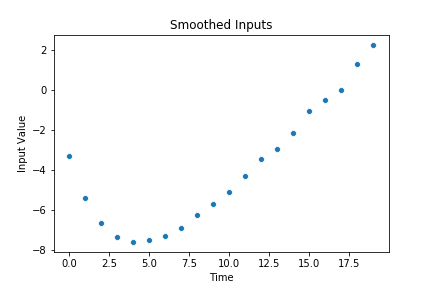
\includegraphics[scale=1.2]{smoothed_inputs.png}
    \caption{Smoothest inputs to achieve $x(20) = 0$ for our linear dynamical system. This achieves $J_{\text{smooth}} = 1.1246$.}
    \label{fig:smoothed_inputs}
  \end{figure}

\newpage
  \Q{Minimum fuel and minimum peak input solutions.}
  \begin{solution}
    First, we verify the inequality $w^Tv \leq ||v||_{\infty}||w||_1$ for $v,w \in \mathbb{R}^p$. We have:
    \begin{align*}
      w^Tv &= \sum_{i=1}^p w_i v_i \tag{Definition of dot product} \\
      &\leq \sum_{i=1}^p |w_i||v_i| \tag{Sum of absolutes must be larger or equal} \\
      &\leq \max_{i=1,\cdots,p}|v_i| \sum_{i=1}^p |w_i| \tag{Multiply by the max $v_i$ instead of each $v_i$} \\
      &= ||v||_{\infty}||w||_1 \tag{Definition of norms}
    \end{align*}
    If we let $z \in\mathbb{R}^n$ be any solution of $Az = y$, and let $\lambda \in \mathbb{R}^m$ be such that $A^T\lambda \neq 0$, then using $z = w \in \mathbb{R}^n$ and $v = A^T\lambda \in \mathbb{R}^n$, by the inequality we just proved, we must have:
    \begin{align*}
      ||z||_1 &\geq \frac{z^T(A^T\lambda)}{||A^T\lambda ||_{\infty}} \tag{By inequality just proved} \\
      &=  \frac{\lambda^TAz}{||A^T\lambda ||_{\infty}} \tag{Numerator is one-dimensional, so its transpose is equal to itself} \\
      &= \frac{\lambda^Ty}{||A^T\lambda ||_{\infty}} \tag{Using $y = Az$}
    \end{align*}
    Therefore, if we can find a vector $x_{\text{mf}} \in \mathbb{R}^n$ and $\lambda \in \mathbb{R}^m$ such that it both (1) solves $Ax_{\text{mf}} = y$ and (2) $||x_{\text{mf}}||_1 = \frac{\lambda^Ty}{||A^Y\lambda ||_{\infty}}$, we will have found the minimum fuel solution. This is because the solution solves (1), and all other solutions will have a $1$-norm larger than $x_{\text{mf}}$ by (2).

    From the lecture notes, we have the linear system:
    \[
      y = Ax
    \]
    where 
    \begin{align*}
      x &=
        \begin{bmatrix}
          x_1 \\
          x_2 \\
          \vdots \\
          x_{10}
        \end{bmatrix} \in \mathbb{R}^{10}\\
      A &=
        \begin{bmatrix}
          9 + \frac{1}{2} & 8 + \frac{1}{2} & \cdots & \frac{1}{2} \\
          1 & 1 & \cdots & 1
        \end{bmatrix} \in \mathbb{R}^{2 \times 10} \\
      y &=
        \begin{bmatrix}
          p(10) \\
          \dot{p}(10)
        \end{bmatrix}
    \end{align*}
    We wish to show that:
    \[
      x_{\text{mf}} =
        \begin{bmatrix}
          \frac{1}{9} \\
          0 \\
          \vdots \\
          0 \\
          -\frac{1}{9}
        \end{bmatrix} \in \mathbb{R}^{10}
    \]
    Following the hint, we will use $\lambda = \begin{bmatrix} 1 \\ -5 \end{bmatrix}$ to prove that the above solution is the minimum-fuel solution. First, we verify that $x_{\text{mf}}$ is a solution to our system:
    \begin{align*}
      Ax_{\text{mf}} &=
        \begin{bmatrix}
          9 + \frac{1}{2} & 8 + \frac{1}{2} & \cdots & \frac{1}{2} \\
          1 & 1 & \cdots & 1
        \end{bmatrix}
        \begin{bmatrix}
          \frac{1}{9} \\
          0 \\
          \vdots \\
          0 \\
          -\frac{1}{9}
        \end{bmatrix} \\
        &=
          \begin{bmatrix}
            1 \\
            0
          \end{bmatrix} = y
    \end{align*}
    The next step is to verify the norm $||x_{\text{mf}}||_1$ is equal to $\frac{\lambda^T y}{||A^T\lambda ||_{\infty}}$. 
    \begin{align*}
      \frac{\lambda^T y}{||A^T\lambda ||_{\infty} } &= \frac{1}{||
        \begin{bmatrix}
          -4\frac{1}{2} \\
          -3\frac{1}{2} \\
          -2\frac{1}{2} \\
          -1\frac{1}{2} \\
          -\frac{1}{2} \\
          \frac{1}{2} \\
          1\frac{1}{2} \\
          2\frac{1}{2} \\
          3\frac{1}{2} \\
          4\frac{1}{2}
        \end{bmatrix}||_{\infty}} \\
        &= \frac{2}{9} \\
        &= |\frac{1}{9}| + |-\frac{1}{9}| \\
        &=||x_{\text{mf}}||
    \end{align*}
    As argued previously, since $x_{\text{mf}}$ satisfies both properties, it must be the case that it is the minimum-fuel solution.  We also verify in code that the $x_{\text{ls}}$ norm is $0.303$ and the $x_{\text{mf}}$ is $0.2$, which is lower.

    As far as the minimum peak force vector, $x_{\text{mp}}$, a good guess would be:
    \[
      x_{\text{mp}} =
        \begin{bmatrix}
          \frac{1}{25} \\
          \frac{1}{25} \\
          \frac{1}{25} \\
          \frac{1}{25} \\
          \frac{1}{25} \\
          -\frac{1}{25} \\
          -\frac{1}{25} \\
          -\frac{1}{25} \\
          -\frac{1}{25} \\
          -\frac{1}{25} 
        \end{bmatrix}
    \]
    Using a similar argument as before, we can verify the above is the mimum peak force vector by verifying that (1) it is a solution such that $Ax_{\text{mp}} = y$ and that the following equality holds, for some $\lambda \in \mathbb{R}^m$ such that $A^T\lambda \neq 0$ (in our case, we use $\lambda = \begin{bmatrix} 1 \\ -5 \end{bmatrix})$:
    \[
      ||x_{\text{mp}}||_{\infty} = \frac{\lambda^T y}{||A^Ty||_{1}}
    \]
    This is because, using the inequality proved previously, we have that for any solution $Az = y$ must have the following hold true:
    \[
    ||z||_{\infty} \geq \frac{\lambda^T y}{||A^T\lambda||_1}
    \]
    See the attaced code, but it is easy for use to verify that $x_{\text{mp}}$ is a valid solution to our system. Furthermore, we can also readily verify that:
    \begin{align*}
      \frac{\lambda^T y}{|| A^T \lambda ||_1} &= \frac{1}{||\begin{bmatrix}
          -4\frac{1}{2} \\
          -3\frac{1}{2} \\
          -2\frac{1}{2} \\
          -1\frac{1}{2} \\
          -\frac{1}{2} \\
          \frac{1}{2} \\
          1\frac{1}{2} \\
          2\frac{1}{2} \\
          3\frac{1}{2} \\
          4\frac{1}{2}
        \end{bmatrix}||_{1}} \\
        &= \frac{1}{9 + 7 + 5 + 3 + 1} \\
        &= \frac{1}{25} \\
        &= ||x_{\text{mf}}||_{\infty}
    \end{align*}
  \end{solution}

  \newpage
  \Q{Singularity of the KKT matrix}
  \begin{solution}
    \begin{enumerate}[label=(\alph*)]
      \item
        Let us suppose that $C \in \mathbb{R}^{k \times n}$ is not full rank. Then we have the following:
        \begin{align*}
          \text{dim}(\textbf{Img}(C^T)) &= \text{dim}(\textbf{Ker}(C))^{\perp} \tag{Property of orthogonal complement and transpose} \\
          &= n - \text{dim}(\textbf{Ker}(C)) \tag{Definition of complement space} \\
          &= n - (n - \text{dim}(\textbf{Img}(C))) \tag{Rank-nullity theorem} \\
          &= \text{dim}(\textbf{Img}(C)) \\
          &< k \tag{$C$ is assumed to not be full-rank}
        \end{align*}
        The above shows that the rows of $C$ must be linearly-dependent (there are $k$ rows, but they don't span a $k$-dimensional space). Therefore, the last $k$ columns $\begin{bmatrix} C^T \\ 0 \end{bmatrix}$ of the KKT matrix are not linearly independent, which means the KKT matrix is singular.
      \item 
        Let us suppose that we have a $u \in \mathbb{R}^n$ such that $u \in \textbf{Ker}(A) \cap \textbf{Ker}(C)$. Then note the following:
        \begin{align*}
          \begin{bmatrix}
            A^TA & C^T \\
            C & 0 
          \end{bmatrix}
          \begin{bmatrix}
            u \\ 0
          \end{bmatrix} &=
          \begin{bmatrix} 
            A^TAu \\
            Cu \\
          \end{bmatrix} \\
          &=
            \begin{bmatrix}
              0 \\ 0
            \end{bmatrix}
        \end{align*}
        As such, we have a non-zero vector in the nullspace of the KKT matrix, therefore the KKT matrix is non-sigular.
      \item
        For this part, let us suppose that $K$ is singular. This means that there exists a nonzero vector $\begin{bmatrix} u \\ v \end{bmatrix} \in \mathbb{R}^{n + k}$ such that:
        \[
          \begin{bmatrix}
            A^TA & C^T \\
            C & 0
          \end{bmatrix}
          \begin{bmatrix}
            u \\ v
          \end{bmatrix} = 0
        \]
        From the above, we have the following two equations:
        \begin{align*}
          A^TAu + C^Tv &= 0 \\
          Cu &= 0
        \end{align*}
        We can immediately conclude that $u \in \text{null}(C)$. Taking the second equation and multiplying on the left by $u^T$, we have:
        \begin{align*}
          u^TA^TAu + u^TC^Tv &= (Au)^T(Au) + (Cu)^Tv \\
          &= (Au)^T(Au) + 0 \tag{$Cu = 0$} \\
          &= ||Au||^2 \\
          &= 0\\
          \implies ||Au|| &= 0 \\
          \implies u &\in \text{null}(A)
        \end{align*}
        Suppose $u \neq 0$, then by the arguments above, we have shown that $u \in \text{null}(A)$ and $u \in \text{null}(C)$, which implies $\text{null}(A) \cap \text{null}(C) \neq \{0\}$. On the other hand, if $u = 0$, then we must have $A^TAu + C^Tv = 0 \implies C^Tv = 0$ with $v \neq 0$. This implies $C$ is not full rank.
    \end{enumerate}
  \end{solution}

  \newpage
  \Q{Portfolio selection with sector neutrality constraints}
  \begin{solution}
    \begin{enumerate}[label=(\alph*)]
      \item 
        We begin by rewriting this problem in matrix form as a minimization subject to some constraints. Our problem, stated directly from the problem statement, is to:
        \begin{align*}
          \text{maximize} & & \mu^Tx - \lambda R^{\text{id}} \\
          \text{subject to} & & \textbf{1}^Tx = 1, Fx = 0
        \end{align*}
        If we define the matrix $\Sigma \in \mathbb{R}^{n \times n}$ where $\Sigma_{ii} = \sigma_i^2$ and $\Sigma_{ij} = 0$, and flipping the maximization to minimization, the problem becomes:
        \begin{align*}
          \text{minimize} & & \lambda x^T\Sigma x -  \mu^Tx  \\
          \text{subject to} & & \textbf{1}^Tx = 1, Fx = 0
        \end{align*}
        To solve the above, we can use Lagrance multipliers. We introduce $a \in \mathbb{R}$ and $b \in \mathbb{R}^k$ ($k + 1$) multipliers, giving us the Lagragian as:
        \[
          L(x, a, b) = \lambda x^T\Sigma x -  \mu^Tx + b^TFx + a(\textbf{1}^Tx - 1)
        \]
        Taking partial derivatives of the above and setting equal to zero gives us the following set of equations:
        \begin{align*}
          \nabla_x L &= 2\lambda\Sigma x - \mu + F^Tb + a\textbf{1} &= 0 \\
          \nabla_a L &= \textbf{1}^Tx - 1 & = 0\\
          \nabla_b L &= Fx &= 0
        \end{align*}
        The above can be written in block-matrix form as:
        \[
          \begin{bmatrix}
            2\lambda \Sigma & \textbf{1} & F^T \\
            \textbf{1}^T & 0 & 0 \\
            F & 0 & 0
          \end{bmatrix}
          \begin{bmatrix}
            x \\
            a \\
            b
          \end{bmatrix}
          = 
          \begin{bmatrix}
            \mu \\
            1 \\
            0
          \end{bmatrix}
        \]

    Finding the optimal $x$ consists of solving this set of linear equations, using the techniques we've learned in class.
    \item
      Using the data in ``sector\_neutral\_portfolio\_data.m'', we find the optimal portofolio $x$ using the above technique. See the code for details. The return associated with this portfolio is 
      \[
        r = 26.706275038813430
      \]
      with idiosyncratic risk:
      \[
      R^{\text{id}} = 133.6297240848970
      \]
    \end{enumerate}
  \end{solution}

  \newpage
  \Q{A simple population model}
  \begin{solution}
    We express the given population dynamics model as an autonomous linear system with state $x(t) \in \mathbb{R}^3$ and state matrix $A \in \mathbb{R}^{3 \times 3}$. We have:
    \[
      \begin{bmatrix}
        x_1(t+1) \\
        x_2(t+1) \\
        x_3(t+1) 
      \end{bmatrix} =
      \begin{bmatrix}
        0 & 2 & 1 \\
        0.6 & 0 & 0 \\
        0 & 0.7 & 0
      \end{bmatrix}
      \begin{bmatrix}
        x_1(t) \\
        x_2(t) \\
        x_3(t)
      \end{bmatrix}
    \]
  \end{solution}


  \newpage
  \Q{Controlling a system using the initial conditions}
  \begin{solution}
    We begin by plugging in the parameters given. This gives us the matrix:
    \[
      A =
        \begin{bmatrix}
          0 & 0 & 1 & 0 \\
          0 & 0 & 0 & 1 \\
          -2 & 1 & 0 & 0 \\
          1 & -1 & 0 & 0
        \end{bmatrix}
    \]
    The solution to this lineary dynamical system at time $t$ is given immediately by the formula:
    \[
      x(t) = e^{tA}x(0)
    \]
    where $x(0) = \begin{bmatrix} 0 \\ 0 \\ \alpha_1 \\ \alpha_2 \end{bmatrix}$
    We use this results in each of the following problems. As such, note that the first two entries of $x(0)$ are always $0$. This means we can drop the first two columns of $e^{tA}$ when solving the system. We call this matrix $E \in \mathbb{R}^{4 \times 2}$. Then our initial state is simply $\alpha = \begin{bmatrix} \alpha_1 \\ \alpha_2 \end{bmatrix} \in \mathbb{R}^2$.
    \begin{enumerate}[label=(\alph*)]
      \item
        In this case, we want to solve the system such that $q_2(10) = 2$. We therefore have the restriction:
        \begin{align*}
          2 &= q_2(10) \\
          &= e_2^Tx(10) \\
          &= e_2^TE\alpha
        \end{align*}
        This is a system with two-variables and only one equation. As such, finding the least-norm solution can be done immediately. We know these variables satisfy our constraints exactly, and we use the additional variable to minimize the norm.
        \[
          \alpha = E_2^T(E_2E_2^T)^{-1}2
        \]
        where $E_2$ is the second row of our matrix $E$. Solving in code, we have:
        \[
          \alpha =
            \begin{bmatrix}
             2.46135192 \\ -9.46473528
            \end{bmatrix}
        \]
      \item
        In this case, we want to solve the system such that $q_1(10) = 1$ and $q_2(10) = 2$. As such, we have the system:
        \[
          \begin{bmatrix}
            1 \\
            2
          \end{bmatrix} = 
          \begin{bmatrix}
            E_1 \\
            E_2
          \end{bmatrix} \alpha
        \]
        This is a system with two equations and two variables, and as such, this specification is feasible. In fact, we can check that our matrix is invertible, and as such, the one and only solutions is given by:
        $$
          \alpha = \begin{bmatrix} E_1 \\ E_2 \end{bmatrix}^{-1}\begin{bmatrix} 1\\ 2 \end{bmatrix}
        $$
        This gives us:
        \[  
          \alpha = 
          \begin{bmatrix}
            -6.44083425 \\
            -11.77979348
          \end{bmatrix}
        \]
        which is the unique solution.
      \item In this case, we have the system:
      \[
        \begin{bmatrix}
          1 \\
          2 \\
          0 \\
          0
        \end{bmatrix} = E\alpha
      \]
      In this case, we have four equations with just two unknowns. As such, this system is not feasible. Instead, we can find the $\alpha$ that comes closest to satisfying the system in the least-squares sense. This is given by:
      \[
        \alpha = (E^TE)^{-1}E^T \begin{bmatrix} 1 \\ 2 \\ 0 \\ 0 \end{bmatrix}
      \]
      which gives us:
      \[
        \alpha =
          \begin{bmatrix}
            -0.13614458 \\
            -0.34345832
          \end{bmatrix}
      \]
      with RMSE of $2.204944721263555$.
      \item These restriction actually give rise to an interesting set of equations. We have our matrix $E \in \mathbb{R}^{4 \times 2}$ as before. Additional, we compute a matrix $E' \in \mathbb{R}^{4 \times 2}$ using the same process but with the new parameters of $m_1 = 1, m_2 = 1.3, k_1 = k_2 = 1$. Then our set of equations can be written as:
      \[
        \begin{bmatrix}
          q_2(10)\\
          q_2(10)
        \end{bmatrix} =
        \begin{bmatrix}
          2\\
          2
        \end{bmatrix} = 
        \begin{bmatrix}
          E_2 \\
          E'_2
        \end{bmatrix}
        \alpha
      \]
      This is a system of two equations with two unknowns. It turns out that the matrix above is a $2 \times 2$ invertible matrix, so there exists one unique solution to this specification given by:
      \[
        \alpha = \left(\begin{bmatrix}
          E_2 \\
          E'_2
        \end{bmatrix} \right)^{-1} \begin{bmatrix}
          2\\
          2
        \end{bmatrix}
      \]
      Computing the above, we have:
      \[
        \alpha =
          \begin{bmatrix}
            10.78304166 \\
            -7.30063808
          \end{bmatrix}
      \]
    \end{enumerate}
  \end{solution}
\end{questions}


\includepdf[
    %% Include all pages of the PDF
    pages=-,
    %% make this page have the usual page style
    %% (you can change it to plain etc). By default pdfpages
    %% sets the pagecommand to \pagestyle{empty}
    pagecommand={\pagestyle{headings}}]
%% The pdf file itself
{HW5Code.pdf}














\end{document}
